%%% The main file. It contains definitions of basic parameters and includes all other parts.

%%% Settings for single-side (simplex) printing
%% Margins: left 40mm, right 25mm, top and bottom 25mm
%% (but beware, LaTeX adds 1in implicitly)
%\documentclass[12pt,a4paper,usenames]{report}
%\setlength\textwidth{145mm}
%\setlength\textheight{247mm}
%\setlength\oddsidemargin{15mm}
%\setlength\evensidemargin{15mm}
%\setlength\topmargin{0mm}
%\setlength\headsep{0mm}
%\setlength\headheight{0mm}
%% \openright makes the following text appear on a right-hand page
%\let\openright=\clearpage

%% Settings for two-sided (duplex) printing
 \documentclass[12pt,a4paper,twoside,openright]{report}
 \setlength\textwidth{145mm}
 \setlength\textheight{247mm}
 \setlength\oddsidemargin{14.2mm}
 \setlength\evensidemargin{0mm}
 \setlength\topmargin{0mm}
 \setlength\headsep{0mm}
 \setlength\headheight{0mm}
 \let\openright=\cleardoublepage

 \raggedbottom

%%disable overfull lines and disable hphenation
%%\usepackage[none]{hyphenat}
%\usepackage[english]{babel}
%\selectlanguage{english}
%\usepackage{hyphenat}
%\allowhyphens
%%\overfullrule=0mm
\hfuzz=5mm
\setlength{\emergencystretch}{10pt}


\interfootnotelinepenalty=10000


\DeclareTextFontCommand{\ttt}{\ttfamily\hyphenchar\font=45\relax}
\DeclareTextFontCommand{\trm}{\rmfamily\hyphenchar\font=45\relax}

%\renewcommand{\baselinestretch}{1.5}

%% Character encoding: usually latin2, cp1250 or utf8:
\usepackage[utf8]{inputenc}


%% Further useful packages (included in most LaTeX distributions)
%\usepackage{amsmath}        % extensions for typesetting of math
\usepackage{amsfonts}       % math fonts
\usepackage{amsthm}         % theorems, definitions, etc.
\usepackage{thmtools}
\usepackage{bbding}         % various symbols (squares, asterisks, scissors, ...)
\usepackage{bm}             % boldface symbols (\bm)
\usepackage{graphicx}       % embedding of pictures
\usepackage{fancyvrb}       % improved verbatim environment
\usepackage{natbib}         % citation style AUTHOR (YEAR), or AUTHOR [NUMBER]
\usepackage[nottoc]{tocbibind} % makes sure that bibliography and the lists
			    % of figures/tables are included in the table
			    % of contents
\usepackage{dcolumn}        % improved alignment of table columns
\usepackage{booktabs}       % improved horizontal lines in tables
\usepackage{paralist}       % improved enumerate and itemize
\usepackage[usenames]{xcolor}  % typesetting in color

\usepackage{tikz}
\usepackage{placeins}
%\usepackage{animate}
\usepackage{float}
\usetikzlibrary{shapes,snakes,arrows,chains}
\usepackage{amsmath}
\usepackage{rotating}

\usepackage{dirtytalk}

\usepackage{dirtree}
\usepackage{url}

\usepackage{longtable}
%%% Basic information on the thesis

% Thesis title in English (exactly as in the formal assignment)
\def\ThesisTitle{SIMD code generator}

% Author of the thesis
\def\ThesisAuthor{Karel Tuček}

% Year when the thesis is submitted
\def\YearSubmitted{2016}

% Name of the department or institute, where the work was officially assigned
% (according to the Organizational Structure of MFF UK in English,
% or a full name of a department outside MFF)
\def\Department{Department of Software Engineering}

% Is it a department (katedra), or an institute (ústav)?
\def\DeptType{Department}

% Thesis supervisor: name, surname and titles
\def\Supervisor{RNDr. David Bednárek, Ph.D.}

% Supervisor's department (again according to Organizational structure of MFF)
\def\SupervisorsDepartment{Department of Software Engineering}

% Study programme and specialization
\def\StudyProgramme{Computer Science}
\def\StudyBranch{General Computer Science}

% An optional dedication: you can thank whomever you wish (your supervisor,
% consultant, a person who lent the software, etc.)
\def\Dedication{%
}

% Abstract (recommended length around 80-200 words; this is not a copy of your thesis assignment!)
\def\Abstract{%
The center of our interest is a problem of pipelined realisation of a special case of data processing networks. These realisations are supposed to realise some computations on series of independent data sets while utilizing SIMD instructions. The aim of this paper is to theoretically investigate the possibilities and the problems of employment of control flow in these networks and also to implement a general framework suitable for generation of these realisations.

The main idea is utilisation of an algorithm crawling over partitions of a network factorised with respect to its control flow. Our idea is that SIMD parallelism should take place on the same instruction realised across multiple data sets.

We illustrate the problems relevant to employment of branching and loops in these networks. We especially discuss a problem of data ordering and also provide relevant proofs. In the analytical part, we show implementation of a general framework which we believe to be suitable for processing of these networks. We also provide examples utilising Intel's SIMD Streaming Extensions.
}

% 3 to 5 keywords (recommended), each enclosed in curly braces
\def\Keywords{%
  {Processing networks} {SIMD} {Parallelism}
}

%% The hyperref package for clickable links in PDF and also for storing
%% metadata to PDF (including the table of contents).
\usepackage[pdftex,unicode]{hyperref}   % Must follow all other packages
\hypersetup{breaklinks=true}
\hypersetup{pdftitle={\ThesisTitle}}
\hypersetup{pdfauthor={\ThesisAuthor}}
\hypersetup{pdfkeywords=\Keywords}
\hypersetup{urlcolor=blue}

% Definitions of macros (see description inside)
%%% This file contains definitions of various useful macros and environments %%%
%%% Please add more macros here instead of cluttering other files with them. %%%

%%% Minor tweaks of style

% These macros employ a little dirty trick to convince LaTeX to typeset
% chapter headings sanely, without lots of empty space above them.
% Feel free to ignore.
\makeatletter
\def\@makechapterhead#1{
  {\parindent \z@ \raggedright \normalfont
   \Huge\bfseries \thechapter. #1
   \par\nobreak
   \vskip 20\p@
}}
\def\@makeschapterhead#1{
  {\parindent \z@ \raggedright \normalfont
   \Huge\bfseries #1
   \par\nobreak
   \vskip 20\p@
}}
\makeatother

% This macro defines a chapter, which is not numbered, but is included
% in the table of contents.
\def\chapwithtoc#1{
\chapter*{#1}
\addcontentsline{toc}{chapter}{#1}
}

% Draw black "slugs" whenever a line overflows, so that we can spot it easily.
\overfullrule=1mm

%%% Macros for definitions, theorems, claims, examples, ... (requires amsthm package)

\declaretheoremstyle[bodyfont=\slshape,spaceabove=12pt]{mystyle}
%headpunct={}
\theoremstyle{mystyle}
\newtheorem{thm}{Theorem}
\newtheorem{theorem}{Theorem}
\newtheorem{lemma}[thm]{Lemma}
\newtheorem{claim}[thm]{Claim}

\newtheorem{observation}{Observation}
\newtheorem{problem}{Problem}
\newtheorem{define}{Definition}
\newtheorem{alg}{Algorithm}
\newtheorem*{defstyle}{}

\theoremstyle{remark}
\newtheorem*{rem}{Remark}
\newtheorem*{cor}{Corollary}
\newtheorem*{example}{Example}

\newcommand{\mybeginfigindent}{\begin{figure}[H]\hspace*{5in}}

\newcommand{\mybeginfigloose}{\begin{figure}[h]}
\newcommand{\mybeginfig}{\begin{figure}[H]}
\newcommand{\myendfig}[2]{\caption{#2}\label{fig:#1}\end{figure}}

\newcommand{\mybegindef}[2]{\begin{define}[#2]\label{def:#1}}
\newcommand{\myenddef}{\end{define}}

\newcommand{\mybeginalg}[2]{\begin{alg}[#2]\label{alg:#1}}
\newcommand{\myendalg}{\end{alg}}

\newcommand{\mybeginprob}[2]{\begin{problem}[#2]\label{pro:#1}}
\newcommand{\myendprob}{\end{problem}}

\newcommand{\mybeginobs}[2]{\begin{observation}[#2]\label{obs:#1}}
\newcommand{\myendobs}{\end{observation}}

\newcommand{\mybeginclaim}[2]{\begin{claim}[#2]\label{cla:#1}}
\newcommand{\myendclaim}{\end{claim}}

%\newcommand{\myexpr}[1]{ $\begin{gathered}[t]\begin{aligned} #1 \end{aligned}\end{gathered}$ }

\newcommand{\myquote}[2]{\\ \\ \centerline{\sl{``#1''}\cite{#2}}}
\newcommand{\myloosequote}[2]{{\sl{``#1''}\cite{#2}}}

%\newcommand{\algref}[1]{\begin{alg}[#1]\end{alg}}
\newcommand{\algref}[1]{\subsubsection{#1}}

\makeatletter
\def\upcase{\expandafter\makeupcase}
\def\makeupcase#1{\uppercase{#1}}

\newcommand{\myexpr}[1]{ $ #1 $ }
  %\newcommand{\mf}[1]{\bm{#1}} 
  \newcommand{\mf}[1]{\mathit{\makeupcase#1}} 

\newcommand{\allowpg}[1]{ \end{code}\ \begin{code} }

\newcommand{\gt}{ > }
\newcommand{\lt}{ < }


%tree items
%\usetikzlibrary{shadows}
%\newcommand{\treelist}{\tikz[overlay]\draw(-.2,-.2)--(-.2,.5) (-.2,.15)--(.1,.15);}
%\newcommand{\treeitem}{\item[\treelist]}
%\newcommand{\treeendlist}{\tikz[overlay]\draw(-.2,-.2)--(-.2,.15) --(.1,.15);}
%\newcommand{\treeend}{\item[\treeendlist]}

%\newcommand{\begincodefig}[2]{\begin{figure}[H]\caption{#2}\label{fig:#1}\begin{code}}
%\newcommand{\endcodefig}{\end{code}\end{figure}}


%moje pridavky
\newcommand{\graphplain}[1]{\begin{figure}[H]\centering\input{contents/graphs/final/#1}\end{figure}}
\newcommand{\graph}[2]{\begin{figure}[H]\centering\input{contents/graphs/final/#1}\caption{#2}\label{fig:#1}\end{figure}}
\newcommand{\graphfloating}[2]{\begin{figure}[h]\centering\input{contents/graphs/final/#1}\caption{#2}\label{fig:#1}\end{figure}}
%\newcommand{\graph}[1]{\begin{figure}[H]\centering\resizebox{.9\linewidth}{!}{\input{contents/graphs/final/#1}}\end{figure}}
  \newcommand{\graphn}[2]{\begin{sidewaysfigure}\resizebox{1\linewidth}{!}{\input{contents/graphs/final/#1}}\caption{#2}\end{sidewaysfigure}}
%k\newcommand{\graph}[1]{\input{contents/graphs/final/#1}\end{figure}}
%k\resizebox{.9\linewidth}{!}{\input{plot.tex}}
\newcommand{\parspace}{\vspace{1\baselineskip}}

%%% An environment for proofs

%%% FIXME %%% \newenvironment{proof}{
%%% FIXME %%%   \par\medskip\noindent
%%% FIXME %%%   \textit{Proof}.
%%% FIXME %%% }{
%%% FIXME %%% \newline
%%% FIXME %%% \rightline{$\square$}  % or \SquareCastShadowBottomRight from bbding package
%%% FIXME %%% }

%%% An environment for typesetting of program code and input/output
%%% of programs. (Requires the fancyvrb package -- fancy verbatim.)


\DefineVerbatimEnvironment{loosecode}{Verbatim}{fontsize=\small, frame=leftline, fontshape=n, samepage=false} 
\DefineVerbatimEnvironment{code}{Verbatim}{fontsize=\small, frame=leftline, fontshape=n, samepage=true} 
\newcommand{\maybreak}[1]{\allowbreak}

\newcommand{\incode}[1]{ \\ \centerline{\texttt{#1}} \\ }

%%% The field of all real and natural numbers
\newcommand{\R}{\mathbb{R}}
\newcommand{\N}{\mathbb{N}}
\newcommand{\arrow}{\rightarrow}
\newcommand{\powerset}{\raisebox{.15\baselineskip}{\Large\ensuremath{\wp}}}

%%% Useful operators for statistics and probability
\DeclareMathOperator{\pr}{\textsf{P}}
\DeclareMathOperator{\E}{\textsf{E}\,}
\DeclareMathOperator{\var}{\textrm{var}}
\DeclareMathOperator{\sd}{\textrm{sd}}

%%% Transposition of a vector/matrix
\newcommand{\T}[1]{#1^\top}

%%% Various math goodies
\newcommand{\goto}{\rightarrow}
\newcommand{\gotop}{\stackrel{P}{\longrightarrow}}
\newcommand{\maon}[1]{o(n^{#1})}
\newcommand{\abs}[1]{\left|{#1}\right|}
\newcommand{\dint}{\int_0^\tau\!\!\int_0^\tau}
\newcommand{\isqr}[1]{\frac{1}{\sqrt{#1}}}

\newcommand{\uv}[1]{``#1''}

%%% Various table goodies
\newcommand{\pulrad}[1]{\raisebox{1.5ex}[0pt]{#1}}
\newcommand{\mc}[1]{\multicolumn{1}{c}{#1}}


% Title page and various mandatory informational pages
\begin{document}
\include{title}

%%% A page with automatically generated table of contents of the bachelor thesis

\tableofcontents

%%% Each chapter is kept in a separate file
\setlength{\parskip}{4mm plus2mm minus2mm}
\include{preface}
\chapter{Theoretical analysis and solution}

    \section{Motivation, the bobox environment}

    %define a box

    \section{Code generation}

        \subsection{Initial definitions} Reader should be familiar with the~basic terminology of the~graph~theory. For now we will assume knowledge of the~following terms: \emph{directed~graph}, \emph{multigraph}, \emph{topological~ordering}, \emph{path}, \emph{cycle}, \emph{connected component}, \emph{depth first search (DFS}. Definitions of these may be found in \cite{kapitoly}. Reader should also be familiar with some basic abbreviation of instruction names and should understand basic concepts of CPU. We will assume knowledge at least of the following abbreviations: \emph{LD (load)}, \emph{ST (store)}, \emph{ADD(+)}, \emph{SIMD (single instruction processing multiple data)}. We will also provide some definitions of our own.

\begin{define}[operation and instruction]
We will use the~term \emph{operation} for general identification of an~operation which is to be performed on some data. The~term \emph{instruction} will be used for a~specific way of performing an~operation. This way, multiple instructions may be associated with a~single operation.
\end{define}

E.g., multiplication by a constant power of two is a~unary operation. Associated instructions may be:
\begin{itemize}
  \item binary shift to left
  \item multiplication using the~asterisk operator
  \item a~vectorized version of multiplication
\end{itemize}

\begin{define}[width of an instruction]
We will use the~term \emph{width} to denote the~number of independent data series a~single instruction operates~on.
\end{define}

\begin{define}[flow graph]
We will use the~term \emph{flow~graph} for any tuple $(G(V,E),O,from:E \arrow \N, to:E \arrow \N, op:V \arrow O)$ which satisfies the~following conditions:
\begin{itemize}
  \item $G(V,E)$ is a~nonempty connected directed acyclic multigraph with annotations defined by $from$, $to$ and $op$.
  \item $O$ is a~set of operations.
  %\item $\forall(v) \in V |out(v)| \leq 1$ 
  \item Any directed edge is uniquely identified by its destination vertex and the~$to$~annotation. I.e.:
    $$ \forall{e=:(a,b),f=:(c,d)} \in {E(G)}: b = d \wedge to(b) = to(d) \Rightarrow e = f $$
\end {itemize}
    We will write $G(V,E)$ for brievity.
\end{define}

This definition of flow graph is almost identical to the definition of \emph{gate networks} given in \cite{ads}, although our use of flow graphs will resemble more the~use of \emph{kahn networks}.

\begin{define}[realization of a flow graph]
  Let $G(V,E)$ be a~flow graph and ${In = \{v \in V \mid |in(v)| = 0\}}$. \emph{Realization~of~a~flow~graph} will be an~algorithm which provided some annotations of outgoing edges of vertices in $In$ produces annotations of all other edges of $G$ such that semantics assigned to $O$ are preserved. 
\end{define}

  Flow graphs will represent pipeline computations. Edges will represent data queues. Vertices will represent data transformations. A~transformation on a \emph{regular} vertex~$v$ will pop exactly one element from every incoming queue of $v$ and push exactly one element into every outgoing queue of $v$. Element pushed into an~outgoing queue~$e$~of~$v$ will be determined from the~elements taken from the~incoming queues~of~$v$, their~$to$~annotations, the~annotation~$op(v)$ and the~annotation~$from(e)$. The~$to$~annotation identifies arguments for operations represented by members~of~$O$. The~$to$~annotation identifies outputs of operations which return more than one value.

\parspace

Note that this scheme describes semantics of every single data serie separately. 

\parspace

Also, note that our definition~of~flow~graph does neither~require nor~ensure semantics~of~$O$ to be consistent. Thus, some flow~graphs may have no realization. We will implicitly assume our flow~graphs to~be consistent with some~semantics assigned~to~$O$. This semantics will always be~clear from their context.



        \subsection{Simple code generation} Consider the~following problem.

\begin{problem}[simple code generation]
Let $G(V,E)$ be a~flow~graph. Let $O$ denote some subset of arithmetic operations of~the~C~language. Also, let $G$ be~consistent with the~semantics of these operations. We wish to~generate a~C~code which will~ realize the~graph~$G$.
\end{problem}

\FloatBarrier

Solution to this~problem is straightforward. First, we order vertices~of~$G$ topologically. Then we take vertices in this order and process them one~by~one. For every vertex~$v$ we use its~annotation to transform its~input~data into its~output~data. Then we save the~output~data under some unique identifier for~later~use.

\parspace

We provide graph representation and resulting code of an~adder~box, which simply loads two values, adds them and stores the~result.

\graph{adder}

\begin{code}
int var_a = input_0[i];
int var_b = input_1[i];
int var_c = a + b;
output_0[i] = c;
\end{code}

\FloatBarrier

We may have noticed that vertices are basically of three types, each of some typical form. 

\begin{itemize}
  \item Input -- \emph{``\textless type\textgreater  \textless variable name\textgreater  = \textless load expression\textgreater ;''}
  \item Output -- \emph{``\textless store expression\textgreater ;''}
  \item Operation -- \emph{``\textless type\textgreater  \textless variable name\textgreater  = \textless operation\textgreater (\textless argument 1\textgreater , \textless argument 2\textgreater );''}
\end{itemize}

This allows us to construct simple patterns which may be~used for actual~code~generation. These may~be the~following:

\begin{itemize}
  \item Input -- \emph{``\$type \$name = \$input;''}
  \item Operation -- \emph{``\$type \$name = \$operation;''}
  \item Output -- \emph{``\$output;''}
\end{itemize}

Where $\$input$ and $\$output$ evaluate to environment-dependent expressions, $\$name$ evaluates to a~new~identifier and $\$operation$ evaluates to a~pattern identified~by the~$op$~annotation. The operation pattern may~contain $\$arg1$, $\$arg2$, $\$arg3$... expressions. These evaluate to the~saved~names from incoming vertices.

\parspace

This scheme~of~generation is actually used --- our generator will~be driven by a~quite complex text-processing system, which will be~based on~recursive evaluation of~shell-like variables in~broader contexts provided~by various extensions.

 %describe the dollar notation

        \subsection{Vectorized code generation} \input{contents/vectorized_generation}

    \section{Handling control flow} At this point we would like to introduce control flow into our pipelines. We shall do so by introducing three new types of operations. These will not be required to fullfill the condition that an operation has to pop/push the same amount of data to/from every queue. 


\begin{define}[node types]
  We shall distinguish the following types of operations:
\begin{itemize}
  \item \emph{regular operation} will be an operation whose semantics is taking one element from every incoming queue of a vertex and pushing one element into every outgoing queue of this vertex. Data to be pushed into an outgoing queue may depend only on the input data and the from annotation of the outgoing queue.
  \item \emph{split operation} will take one data input and one condition input (Boolean value typically). Depending on the condition input it will decide upon exactly one of its outgoing $from$ annotations and push data into all outgoing queues with this annotation. All other outgoing queues will remain unchanged. The data input and the condition input will be consumed.
  \item \emph{merge operation} will take two data inputs and one condition input. Depending on the condition input it will take data from one of the inputs and push them to all output queues. Data in the chosen input and in the condition input will be consumed. All other incoming queues will remain unchanged.

  %Some generation systems may decide against using the condition input and just take data in unspecified order.
  %The observations would not hold with this.
  \item \emph{loop merge operation} will take two data inputs. If there is any data in the second input, this node takes the data from the second input and puts it into all outgoing queues. Otherwise it does the same thing with the first input. Moreover, we will allow the second input to be on cycles, i.e., we will not consider the second input edge when saying \emph{acyclic} or \emph{topological ordering}. By doing this we will not void semantical meaning of flow graphs since standard edges represent data dependencies unlike these edges.
\end{itemize}
\end{define}

Using the standard \emph{split} and \emph{merge} nodes we will be able to perform standard branching, i.e., to realize the \texttt{ if \string{\string} else \string{\string} } construct. The \emph{loop merge} node in combination with the standard \emph{split} node will allow us to realize the \texttt{ while(condition) \string{\string} } construct. We show this in a picture.

\begin{rem}
  Until now we have used only rectangular nodes in our graphs. From now on we will also use circular nodes which will denote connected parts of graphs.
\end{rem}

\graph{cf_constructs}

Until now we have performed all data transformations \emph{regulary}. Thanks to that we did not need to bother ourselves with checking of the consistency of graphs. Now we will have to.

\begin{define}[consistency of a flow graph]
  We shall say that a flow graph $G(V,E)$ with a set of operations $O$ is \emph{consistent} if and only if the following conditions hold:
  \begin{itemize}
    \item Semantics of $O$ are satisfied. That is:
      \begin{itemize}
        \item Counts of incoming and outgoing edges and their $from$ and $to$ annotations match the semantics assigned to $O$.
        \item Data type semantics of $O$ are satisfied.
        \item Any other semantic restrictions of $O$ relating to the graph structure are satisfied. 
      \end{itemize}
    \item Only elements from the same data serie may interfere in any realization of G.
  \end{itemize}
\end{define}


Apparently not all graphs satisfy the second condition. Here is one such graph. Here two values from different data series will be added.

\FloatBarrier

\graph{inconsistent}

\FloatBarrier

We will not present any way of consistency testing of general flow graphs. We will content ourselves with an observation that nontrivial consistent flow graphs exist.

\begin{observation}[consistency of schemas]
  The examples of node type usage are consistent if the following conditions hold:
  \begin{itemize}
    \item Branch or loop bodies, conditions, peamble and epilogue consist only of regular operations.
    \item The branching preamble may be connected with the condition by a regular operation without voiding consistency.
    \item There are no concealed paths inbetween:
      \begin{itemize}
        \item if branch and else branch
        \item any branch and a preamble/condition/epilogue
        \item loop body and loop condition
        \item loop body/condition and a preamble/epilogue
      \end{itemize}
    \item Semantics of $O$ are preserved.
    \end{itemize}
  \begin{proof} 
    Assume that two different data series come into contact. We have banned any direct contact between any two queues which may cause this. Thus, the only thing to consider is the merge and the split node. But flow of data from every split leads to a merge which merges according the same condition, which means that the two data flows are merged in such manner that both order and quantity of the data series is preserved.
  \end{proof}
\end{observation}

\begin{observation}[schema nesting]
  Let $G(V,E)$ with $O$ be a consistent flow graph and $C$ a connected subgraph of $G$ composed only of regular nodes, i.e., of vertices annotated by regular operations. Now we create a new graph by nesting a graph $H$ corresponding to either of the provided example schemas into $C$. We do so by connecting vertices of $C$ and $H$ by edges and by changing some regular operations into another regular operations. Then the new graph is consistent if the following conditions are satisfied:
  \begin{itemize}
    \item The nested schema satisfies the conditions from previous observation.
    \item The nested schema is connected to C only by the preamble and epilogue.
    \item The nested schema does not contain any input operations. (According to our definition of graph realization these are exactly vertices with no input edges)
    \item We have not introduced any new cycle except for cycles containing second input of any loop node.
    \item Semantics of $O$ are preserved.
  \end{itemize}
  \begin{proof} 
    This follows directly from the proof of the previous observation and the structure of $G$.
  \end{proof}
\end{observation}

\begin{observation}[schema sequencing]
  Let $G(V,E)$, $O$ and $C$ be defined as in the previous observation. Now we take one of the example schemas and embed it multiple times into $C$ in the means of the previous observation. If we use the same condition for all inserted instances of the chosen schema, then we may join the corresponding bodies of the embeded schemas without voiding consistency of the new graph.
  \begin{proof} 
    By structure of $G$ using an argument analogical to the proof of the \emph{consistency of schemas}.
  \end{proof}
\end{observation}




        \subsection{Partitioning the graph} At this point we would like to examine possibilities of realization of flow graphs with all 4 types of nodes. 

\parspace

In the previous section we have shown how pipelines composed of regular operations may be processed. This approach does not suffice since different nodes may need to process data at different speeds. 

\parspace

\FloatBarrier

Our strategy is to cut the flow graph into partitions such that every partition consists only of regular operations. Then we add actual buffers between these partitions. The data will then be processed by a crawler which will go through our graph and process its partitions one at a time. Every single partition will be processed by code generated by generators we have already presented. 

\parspace

First, we will need some definitions.

\begin{define}[edge layer]
Let there be a graph (possibly directed multigraph) $G(V,E)$. We will assign one more numeric annotation to every edge. We will call this annotation \emph{layer}. Thus we have $layer: E \arrow \N_0$. If $layer(e) = n$ we will say that $e$ is on layer $n$.
\end{define}

Layer will denote type of edge. It will allow us to talk about subsets of edges in a more intuitive manner and also to introduce a more complex graph structure. We show our visual convention in the following picture.

\graph{lines}

\begin{define}[factor graph]
  Let $G(V,E)$ and $G_f(V_f,E_f)$ be graphs (possibly directed multigraphs). We will say that $G_f$ is a \emph{factor graph} of $G$ if there exists a function $f: V \arrow V_f$ such that:
\begin{itemize}
  \item $f(u) = f(v)$ if and only if there exists an undirected path $P_{u,v}$  in $G$ which uses only edges on layer 0. 
  \item $\exists(e =: (u,v) \in E)(layer(e) = 1) \Longleftrightarrow \exists(e_f \in E_f)( e_f = (f(u), f(v)) )$
\end{itemize}
\end{define}

Note that this definition overrides another meaning of this term.






        \subsection{First proposal - ordered tree crawler} 
\begin{tikzpicture}[>=latex,line join=bevel,]
%%
\begin{scope}
  \pgfsetstrokecolor{black}
  \definecolor{strokecol}{rgb}{0,0,0};
  \pgfsetstrokecolor{strokecol}
  \draw (480bp,443bp) -- (480bp,518bp) -- (798bp,518bp) -- (798bp,443bp) -- cycle;
  \draw (639bp,506bp) node {some partition j \textless i};
\end{scope}
\begin{scope}
  \pgfsetstrokecolor{black}
  \definecolor{strokecol}{rgb}{0,0,0};
  \pgfsetstrokecolor{strokecol}
  \draw [solid] (806bp,80bp) -- (806bp,665bp) -- (1196bp,665bp) -- (1196bp,80bp) -- cycle;
  \draw (1001bp,653bp) node {vectorized code of partition i};
\end{scope}
\begin{scope}
  \pgfsetstrokecolor{black}
  \definecolor{strokecol}{rgb}{0,0,0};
  \pgfsetstrokecolor{strokecol}
  \draw [solid] (8bp,8bp) -- (8bp,665bp) -- (472bp,665bp) -- (472bp,8bp) -- cycle;
  \draw (240bp,653bp) node {singular code of partition i};
\end{scope}
\begin{scope}
  \pgfsetstrokecolor{black}
  \definecolor{strokecol}{rgb}{0,0,0};
  \pgfsetstrokecolor{strokecol}
  \draw (480bp,80bp) -- (480bp,155bp) -- (798bp,155bp) -- (798bp,80bp) -- cycle;
  \draw (639bp,143bp) node {some partition j \textgreater i};
\end{scope}
  \node (sbodylab) at (170bp,253bp) [draw,rectangle] {SINGULAR\_BODY\_i};
  \node (sbody) at (170bp,106bp) [draw,ellipse] {$\begin{matrix} \text{process body} \\ \text{remaining --} \end{matrix}$ };
  \node (vbody) at (991bp,181bp) [draw,ellipse] {$\begin{matrix} \text{process body} \\ \text{remaining -= vector size} \end{matrix}$ };
  \node (inv) at (739bp,469bp) [draw,rectangle] {PARTITION\_j};
  \node (ins) at (579bp,469bp) [draw,rectangle] {SINGULAR\_PARTITION\_j};
  \node (sterm) at (253bp,469bp) [draw,ellipse] {i != 0 ? handle\_termination\_nonzero};
  \node (vrepeat) at (1073bp,106bp) [draw,ellipse] {repeat};
  \node (sgoprev) at (256bp,397bp) [draw,ellipse] {an empty input from j};
  \node (slab) at (170bp,616bp) [draw,rectangle] {SINGULAR\_PARTITION\_i};
  \node (outs) at (579bp,106bp) [draw,rectangle] {SINGULAR\_PARTITION\_j};
  \node (srepeat) at (109bp,34bp) [draw,ellipse] {repeat};
  \node (outv) at (739bp,106bp) [draw,rectangle] {PARTITION\_j};
  \node (vbodylab) at (991bp,253bp) [draw,rectangle] {VECTOR\_BODY\_i};
  \coordinate (aux) at (56bp,469bp);
  \node (sterm0) at (202bp,544bp) [draw,ellipse] {i == 0};
  \node (vlab) at (1067bp,616bp) [draw,rectangle] {PARTITION\_i};
  \coordinate (vaux) at (1160bp,469bp);
  \node (vgonext) at (991bp,325bp) [draw,ellipse] {$\begin{matrix} \text{not enough space} \\ \text{in an output to j} \end{matrix}$ };
  \node (sgovector) at (338bp,253bp) [draw,ellipse] {process vectorized};
  \node (vgoprev) at (992bp,397bp) [draw,ellipse] {$\begin{matrix} \text{not enough data} \\ \text{in an input from j} \end{matrix}$ };
  \node (sgonext) at (170bp,181bp) [draw,ellipse] {afull output to j};
  \node (vterm0) at (994bp,544bp) [draw,ellipse] {i == 0 ? handle\_termination\_zero};
  \node (sgovectorized) at (260bp,325bp) [draw,ellipse] {$\begin{matrix} \text{not enough input or space} \\ \text{for vectorized body} \end{matrix}$ };
  \node (vterm) at (992bp,469bp) [draw,ellipse] {i != 0 \&\& i is terminating};
  \draw [->,very thick] (sterm) -- (sgoprev);
  \draw [->,very thick] (sgovectorized) -- (sgovector);
  \draw [->,dotted] (vgonext) -- (outv);
  \draw [->,dotted] (sterm) -- (outv);
  \draw [->,very thick] (vterm) -- (vgoprev);
  \draw [->,very thick] (sgonext) -- (sbody);
  \draw [<-,dotted] (ins) -- (vgoprev);
  \draw [->,very thick] (vbody) -- (vrepeat);
  \draw [->,very thick] (vterm0) -- (vterm);
  \draw [->,solid] (sterm) -- (sbodylab);
  \draw [->,very thick] (sterm0) -- (sterm);
  \draw [->,very thick] (vbodylab) -- (vbody);
  \draw [->,very thick] (sbody) -- (srepeat);
  \draw [->,solid] (sgovector) -- (vbodylab);
  \draw [->] (sgovectorized) -- (sbodylab);
  \draw [<-,dotted] (ins) -- (sgoprev);
  \draw [] (aux) -- (srepeat);
  \draw [->,dotted] (sgonext) -- (outs);
  \draw [->,very thick] (vgonext) -- (vbodylab);
  \draw [<-] (slab) -- (aux);
  \draw [->,very thick] (slab) -- (sterm0);
  \draw [->,solid] (vterm) -- (slab);
  \draw [] (vaux) -- (vrepeat);
  \draw [->,solid] (vterm0) -- (sbodylab);
  \draw [<-] (vlab) -- (vaux);
  \draw [->,solid] (sterm0) -- (vlab);
  \draw [->,very thick] (sgoprev) -- (sgovectorized);
  \draw [->,very thick] (vlab) -- (vterm0);
  \draw [->,very thick] (vgoprev) -- (vgonext);
  \draw [->,very thick] (sbodylab) -- (sgonext);
  \draw [->,dotted] (vterm0) -- (outv);
%
\end{tikzpicture}



        \subsection{Second proposal - unordered solution} \input{contents/unordered.tex}

        \subsection{Refinement of the second proposal} The unordered solution seems to be superior to the ordered one in many aspects. An optimal situation would of course be if we could drop the condition. Unfortunately the receiver of the processed data may need the data ordered. We of course may add serie indices into the data series for identification, but that does not solve the problem entirely, since either we will have to store the results one by one or someone else will have to retrieve them one by one. Either version would increase the amount of data transfers between CPU and RAM significantly. 

\parspace

Idealy we would like to reorder the data back using as few RAM stores and loads as possible. For this purpose we may use the information about performed shuffling of the data. We propose the following approach:
\begin{enumerate}
  \item Process all data and store results into the RAM. Also store a sequence of boolean values per every split or merge node. This sequence will contain a single value per every data serie which was processed by the node in question. This value will represent either left or right branch of the split or merge.
  \item Construct a new pipeline, which will be an exact copy of the processing pipeline, will be built backwards and will not contain any data processing.
  \item Then pipe the data from RAM into the new pipeline in inverse order. Also provide every split and merge node with the values stored by a corresponding merge or split as a control.
\end{enumerate}

\begin{rem}
  Note that we cannot pipe the original pipeline directly to the one built backwards. Imagine that the first data serie to enter the processing pipeline is the last one to come out. If we piped the first pipeline directly into the sorting one, we would have to store \emph{all} data in CPU registers until the first data serie was processed and could be piped into the sorting pipeline.
\end{rem}

This approach surely has its drawbacks, but for some pipelines may reduce the amount of RAM transfers needed for sorting of the data.


\chapter{General implementation}

    \section{Brief introduction of components}

        \subsection{Command environment}

        \subsection{Instruction Table} 

        \subsection{Graph}

        \subsection{Generator}

        \subsection{Loaders}

        \subsection{Preprocessing environment and the Writer class}

            \subsubsection{Writer}

            \subsubsection{Alias environments}

        \subsection{Alias environments as drivers of the generation}

    \section{Flow example}

    \section{Graph algorithms}

    \section{Instruction representation and actual implementation of the generator}

        %%....

\chapter{Implementation of the SSE instruction set}

    \section{Data types and conversions}

    \section{Considering load and store problems} 

    \section{Actual alias environments} 
      
        %%....

    \section{Control-flow related objects} 

        %%....

\chapter{User guides}

    \section{Commands available}

    \section{Understanding the preprocessor}

    \section{Format specifications}

        \subsection{csv}

        \subsection{xml}

    \section{Detailed field semantics}

    \section{FAQ}
        \subsection{How do I extend or use existing tables/models}

        \subsection{How do I add support for a new language?}

\begin{code}
for i in abc
do
done
\end{code}

\graph{simple}
\graph{simple2}
\graph{cf}




\include{epilog}

%%% Bibliography
\include{bibliography}

%%% Figures used in the thesis (consider if this is needed)
\listoffigures

%%% Tables used in the thesis (consider if this is needed)
%%% In mathematical theses, it could be better to move the list of tables to the beginning of the thesis.
%\listoftables

%%% Abbreviations used in the thesis, if any, including their explanation
%%% In mathematical theses, it could be better to move the list of abbreviations to the beginning of the thesis.
%\chapwithtoc{List of Abbreviations}

%%% Attachments to the bachelor thesis, if any. Each attachment must be
%%% referred to at least once from the text of the thesis. Attachments
%%% are numbered.
%%%
%%% The printed version should preferably contain attachments, which can be
%%% read (additional tables and charts, supplementary text, examples of
%%% program output, etc.). The electronic version is more suited for attachments
%%% which will likely be used in an electronic form rather than read (program
%%% source code, data files, interactive charts, etc.). Electronic attachments
%%% should be uploaded to SIS and optionally also included in the thesis on a~CD/DVD.
\chapwithtoc{Attachments}
\begin{itemize}
  \item Source code of our framework with examples of instruction tables and example implementations of alias environments should be distributed along with electronic version of this thesis. Plain git repository may be found at \url{http://www.ktweb.cz/ctb}. Browsable mirror is to be found at \url{http://www.github.com/kareltucek/ctb}. Description of directory structure may be found in Section \ref{sec:directories}.
\end{itemize}

\openright
\end{document}
